% ============================================================
\chapter{Idzorek の確信度の方法}\label{ch:idzorek}

Idzorek の論文 \textit{A Step-by-Step Guide to the Black-Litterman Model: Incorporating User-Specified Confidence Levels}（初稿 2002 年、2004 年版、2007 年に Satchell 編の本の 1 章として出版）は、BL の入力の作り方を、8 資産の例で 1 段ずつ示した。いまも実務でいちばんよく参照される解説の 1 つである。この論文の新しい提案は、$\Omega$ を「0〜100\% の確信度」から決める方法である。

この章では、論文の例を表の数字どおりに再現し、確信度の方法が閉じた式になることを示す。そのうえで、論文では触れられていない注意点（ビューが複数あると、指定した確信度どおりには比率が動かない）を確かめる。

\section{例の設定}

例の資産は 8 つの資産クラスである。論文の表 5 の共分散（過去 60 か月の超過リターン）と、時価総額の比率を\tabref{tab:idz-inputs}に示す。

\begin{table}[htbp]
\centering
\caption{Idzorek の例の入力（年率 \%）。$\Pi$（論文）は論文の表 1 の値。右端は、論文の表から逆算した $\lambda=\V{idz.lam}$ で $\lambda\Sigma\wmkt$ を計算し直したもの。}
\label{tab:idz-inputs}
\tabin{idz_inputs}
\end{table}

論文は、市場のリスクプレミアム 3\% を市場の分散で割って $\lambda\approx3.07$ としている。逆算した $\lambda=\V{idz.lam}$ で $\Pi$ を計算し直すと、論文の表との差は最大 \V{idz.pidiff}\% で、表の丸めの範囲である。市場の標準偏差は \V{idz.mktsd}\%、期待超過リターンは \V{idz.mktprem}\% になる。

論文はまず、均衡以外の期待リターンを最適化に入れると何が起きるかを見せている。過去 60 か月の平均リターンを使うと、米国債券 1144\%、外国債券 $-105\%$、先進国株式 $-104\%$ という比率になる。回帰のベータの CAPM を使うと、均衡との相関は 99.8\% なのに、比率との相関は 66\% にとどまる。均衡リターン $\Pi$ を使えば、比率は時価総額の比率に戻る。

\section{3 つのビュー}

論文のビューは次の 3 つである。

\begin{enumerate}
\item 先進国株式（米国以外）の超過リターンは 5.25\% になる（確信度 25\%）。
\item 外国債券は米国債券を 0.25\% 上回る（確信度 50\%）。
\item 米国の大型・小型グロースは、米国の大型・小型バリューを 2\% 上回る（確信度 65\%）。
\end{enumerate}

\begin{table}[htbp]
\centering
\caption{3 つのビュー。$p_k\Pi$ は均衡が示すビューの値。$\omega^{\mathrm{HL}}$ は He--Litterman の $\tau p_k\Sigma p_k\T$（$\tau=0.025$）、$\omega^{\mathrm{Idz}}$ は確信度 $C_k$ から決めた値。}
\label{tab:idz-views}
\tabin{idz_views}
\end{table}

\tabref{tab:idz-views} の $p_k\Pi$ と $Q_k$ を比べると、ビューの「向き」が分かる。

\begin{itemize}
\item ビュー 1：均衡は \V{idz.ppi1}\%、ビューは 5.25\% なので、強気のビューである。
\item ビュー 2：均衡の差は \V{idz.ppi2}\%、ビューは 0.25\% なので、外国債券について\textbf{弱気}のビューである。言葉では「外国債券が上回る」だが、均衡が示す差より小さいので、比率は米国債券へ動く。
\item ビュー 3：均衡の差は \V{idz.ppi3}\%、ビューは 2\% なので、これもグロースについて\textbf{弱気}である。
\end{itemize}

ビューの言葉の向きと、比率が動く向きが逆になりうる。ビューは「均衡と比べてどうか」で効く、ということを忘れないようにしたい。

\subsection*{相対ビューの重みの付け方}

ビュー 3 は 4 つの資産を含む。$P$ の行の重みの付け方には 2 つの流儀がある。

\begin{itemize}
\item \textbf{等しい重み}（Satchell and Scowcroft 2000）：グロースの 2 資産に $+0.5$ ずつ、バリューの 2 資産に $-0.5$ ずつ。
\item \textbf{時価総額の重み}（Idzorek）：大型と小型の時価総額は 9 対 1 なので、$+0.9$、$+0.1$、$-0.9$、$-0.1$。
\end{itemize}

等しい重みでは、時価総額が 9 分の 1 しかない小型株の比率が大型株と同じだけ動き、意図しない大きなずれが生じる。Idzorek は時価総額の重みを勧めている。この資料の計算も時価総額の重みを使う。

\section{He--Litterman の $\Omega$ で計算する}

まず、He と Litterman の $\Omega=\diag(\tau p_k\Sigma p_k\T)$（$\tau=0.025$）で計算する。結果を\tabref{tab:idz-result}に示す。

\begin{table}[htbp]
\centering
\caption{事後の期待リターン $\mu$ と比率 $w$（年率 \%）。HL は He--Litterman の $\Omega$、Idz は Idzorek の確信度（25\%、50\%、65\%）から決めた $\Omega$、100\% は $\Omega=0$。比率は制約のない最適化 $w=(\lambda\Sigma)^{-1}\mu$。}
\label{tab:idz-result}
\tabin{idz_result}
\end{table}

HL の列は、論文の表 6 と、期待リターンで最大 \V{idz.erdiff}\%、比率で最大 \V{idz.wdiff}\% の差で一致する。読み取れることを挙げる。

\begin{itemize}
\item 期待リターンは 8 資産すべてで動くが、比率が動くのはビューのある 7 資産だけで、新興国株式は時価総額の比率のままである（\secref{sec:hl-property}）。
\item ビュー 1 は絶対ビューなので、比率の合計が \V{idz.wsum}\% になり、100\% を超える。全額投資の制約がある運用なら、絶対ビューは扱いに注意がいる。
\item 論文の表 8 の事前の指標も再現できる。BL の比率の標準偏差は \V{idz.blsd}\%、時価総額の比率からのずれ（アクティブリスク）は \V{idz.actrisk}\% である。ビューは比率を少ししか動かしていない。
\end{itemize}

\section{黙示の確信度}

Idzorek は、まず「いまの $\Omega$ は、確信度で言うと何 \% に当たるか」を測った。そのために、$\Omega=0$（100\% の確信）のときの比率 $w_{100\%}$ を計算し、
\begin{equation}
\text{黙示の確信度}=\frac{\hat w-\wmkt}{w_{100\%}-\wmkt}
\label{eq:implied-conf}
\end{equation}
を資産ごとに求める。100\% 信じたときの傾きに対して、実際には何割傾いたか、である。

He--Litterman の $\Omega$ では、3 つのビューの黙示の確信度は \V{idz.impl1}\%、\V{idz.impl2}\%、\V{idz.impl3}\% になる（論文では 32.94\%、43.06\%、33.02\%）。ビューを 1 つずつ入れた場合は、どのビューも 50\% である（\V{idz.single}）。ビューが 1 つなら、He--Litterman の $\Omega$ は「確信度 50\%」と同じだ、ということである。3 つ同時に入れると 50\% からずれるのは、ビューどうしが相関していて、互いの効き方に影響するからである。

いずれにせよ、ユーザーが言った確信度（25\%、50\%、65\%）は、He--Litterman の $\Omega$ では無視されている。Idzorek はこれを問題とし、確信度から $\Omega$ を決める方法を提案した。

\section{Idzorek の方法の手順}

ビュー $k$ ごとに、次の手順で $\omega_k$ を決める。

\begin{enumerate}
\item ビュー $k$ だけを 100\% 信じたときの期待リターン $\mu_{k,100\%}=\Pi+\tau\Sigma p_k\T(p_k\tau\Sigma p_k\T)^{-1}(Q_k-p_k\Pi)$ を計算する。
\item その比率 $w_{k,100\%}=(\lambda\Sigma)^{-1}\mu_{k,100\%}$ を計算する。
\item 100\% のときの傾き $D_{k,100\%}=w_{k,100\%}-\wmkt$ を求める。
\item 確信度 $C_k$ を掛けて、目標の傾き $C_k D_{k,100\%}$ を求める。
\item 目標の比率 $w_{k,\%}=\wmkt+C_kD_{k,100\%}$ を求める。
\item ビュー $k$ だけを $\omega_k$ で入れたときの比率 $w_k(\omega_k)$ が、目標の比率にもっとも近くなる $\omega_k$ を探す（差の 2 乗和を最小にする）。
\item すべてのビューの $\omega_k$ を並べて $\Omega$ を作り、BL の公式で事後の期待リターンを計算する。
\end{enumerate}

この手順では $\tau$ の値は結果に効かない。Idzorek はこれを利点として挙げている。

\section{閉じた式になる}\label{sec:idz-closed}

手順 6 は数値で探すように書かれているが、実は答えが式で書ける。ビュー $k$ だけを入れたとき、比率の傾きは式~\eqref{eq:hl-weights} から
\begin{equation}
w_k(\omega_k)-\wmkt=p_k\T\,\frac{\tau}{\lambda}\,\frac{Q_k-p_k\Pi}{\tau p_k\Sigma p_k\T+\omega_k}
\end{equation}
である。$\omega_k=0$ のときとの比は
\begin{equation}
\frac{w_k(\omega_k)-\wmkt}{w_{k,100\%}-\wmkt}=\frac{\tau p_k\Sigma p_k\T}{\tau p_k\Sigma p_k\T+\omega_k}
\end{equation}
で、ビューに含まれるすべての資産で同じ値になる。これが $C_k$ に等しくなるのは
\begin{equation}
\boxed{\;\omega_k=\tau\,p_k\Sigma p_k\T\cdot\frac{1-C_k}{C_k}\;}
\label{eq:idz-closed}
\end{equation}
のときである。目標の比率にちょうど一致するので、手順 6 の差の 2 乗和は 0 になる。この式は Walters の解説（2014）にあり、PyPortfolioOpt の Idzorek の方法も、Walters の閉じた式を使うと説明している。

\begin{exbox}[数値で確かめる]
論文の手順 6 のとおりに数値で $\omega_k$ を探すと、式~\eqref{eq:idz-closed} との差は最大 \V{idz.omnumdiff}\% だった。$\omega_k$ は\tabref{tab:idz-views}の右端の列で、He--Litterman の値と比べると、ビュー 1（確信度 25\%）は \V{idz.omratio1} 倍、ビュー 2（50\%）は \V{idz.omratio2} 倍、ビュー 3（65\%）は \V{idz.omratio3} 倍である。確信度 50\% が He--Litterman と同じになることも確かめられる。
\end{exbox}

式~\eqref{eq:idz-closed} から分かることを挙げる。

\begin{itemize}
\item $C_k$ は、ビューが 1 つのときの採用率 $s$ そのものである（式~\eqref{eq:adoption}）。Idzorek の確信度は「均衡からビューへ何割動かしたいか」を直接言っていることになる。
\item $C_k=50\%$ は He--Litterman と同じ。$C_k\to100\%$ で $\omega_k\to0$、$C_k\to0$ で $\omega_k\to\infty$。
\item $\omega_k$ は $\tau$ に比例するので、$\tau$ は消える。
\end{itemize}

\section{ビューが複数あると、確信度どおりには動かない}\label{sec:idz-multi}

手順 1〜6 は、ビューを 1 つずつ扱っている。手順 7 で 3 つを同時に入れたとき、それぞれのビューの傾きは確信度どおりになるだろうか。式~\eqref{eq:implied-conf} で確かめた結果を\tabref{tab:idz-conf}に示す。

\begin{table}[htbp]
\centering
\caption{黙示の確信度。「1 つだけ」はビューを 1 つずつ入れた場合、「3 つ同時」はすべてを入れた場合。分母の 100\% の傾きは、それぞれ同じ条件（1 つだけ、3 つ同時）で $\Omega=0$ にしたもの。}
\label{tab:idz-conf}
\tabin{idz_conf}
\end{table}

\begin{figure}[htbp]
\centering
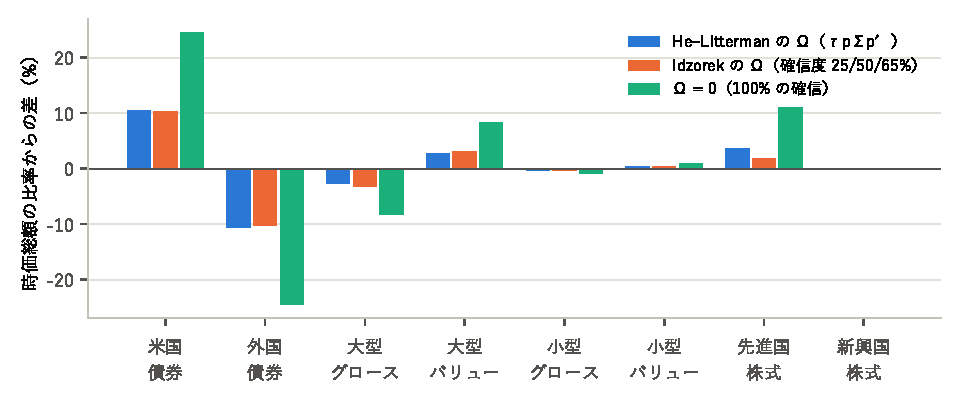
\includegraphics[width=0.95\linewidth]{fig_idz_tilts.pdf}
\caption{3 つのビューを同時に入れたときの、時価総額の比率からの差。Idzorek の $\Omega$（確信度 25/50/65\%）でも、傾きは 100\% のときの 25/50/65\% にはならない。}
\label{fig:idz-tilts}
\end{figure}

3 つを同時に入れると、確信度 25\% のビュー 1 は \V{idz.ach1}\%、50\% のビュー 2 は \V{idz.ach2}\%、65\% のビュー 3 は \V{idz.ach3}\% しか傾かなかった（\figref{fig:idz-tilts}）。指定どおりにならない理由は、事後の式の $(P\tau\Sigma P\T+\Omega)^{-1}$ にある。ビューのポートフォリオどうしが相関していると、この逆行列の非対角成分を通じて、あるビューの驚きが別のビューの傾きを打ち消したり強めたりする。例では、先進国株式（ビュー 1）とグロース・バリューの差（ビュー 3）がどちらも株式で、共分散を持つ。

これは Idzorek の方法の誤りではない。論文は、確信度を「ビューごとの傾きの目安」として決める方法を提案しており、組み合わせたときの傾きまでは約束していない。ただ、利用者は「65\% と言ったのだから 65\% 動く」と考えがちなので、注意がいる。

3 つ同時の傾きを確信度に合わせたいなら、3 つの $\omega_k$ をまとめて探す方法が考えられる。この例で探すと、$\omega=(\V{idz.omjoint1},\ \V{idz.omjoint2},\ \V{idz.omjoint3})\times10^{-4}$ で、3 つのビューの傾きはそれぞれ \V{idz.achj1}\%、\V{idz.achj2}\%、\V{idz.achj3}\% になった（目標との差の最大は \V{idz.joint.res}）。ビュー 3 の $\omega$ はほぼ 0、つまり 100\% の確信まで上げても、傾きは 65\% に届かなかった。ほかのビューとの相関に打ち消されるためで、確信度の組み合わせによっては、3 つを同時に合わせることはできない。

そもそも、確信度は「ビューをどれだけ信じるか」であって、「比率をどれだけ動かすか」ではない。後者に無理に合わせると、相関によって打ち消し合うビューの確信を、根拠なく高く置くことになる（例では 100\% にまで上がった）。比率の動きを確信度に合わせることにこだわらず、確信度は 1 つずつの採用率として決め、組み合わせたときの動きは黙示の確信度で確かめるのがよい。

\section{確信度をどう決めるか}

Idzorek は、確信度を決める材料として、ビューを作ったモデルや分析者の過去の当たり具合、ビューと均衡の差の大きさなどを挙げている。さらに、複数の分析者からビューを集めるなら、それぞれの情報係数（IC、予想と実際の相関）に応じて確信度を決めれば、腕のよい分析者を重く扱える、と述べている（Grinold and Kahn 1999 の IC）。

ここで、確信度を当たり具合から決めると、どんな数字になるかを先に見ておく（詳しくは \chapref{ch:accuracy}）。予想と実際のリターンの相関が IC のとき、予想に合わせて期待リターンを動かすべき割合は、おおよそ $\IC^2$ である。IC は、腕のよい運用者でも 0.05〜0.10 程度とされる（『総合報告書』の Grinold の式の節）。つまり、当たり具合に見合う確信度は 0.25〜1\% である。人が言葉で選ぶ 25\%、50\%、65\% は、当たり具合の点では 2 桁大きい。

\begin{notebox}[確信度の言葉と、当たり具合の数字]
「65\% 確信している」という言葉は、多くの人にとって「かなり自信がある」程度の意味である。しかし BL の確信度は「均衡からビューへ 65\% 動かす」という意味になる。来月のリターンの予想で、均衡から 65\% 動かしてよいほど当たる予想は、ほとんどない。確信度を言葉で決めるときは、その値が採用率として妥当かを、当たり具合の数字（IC）と照らし合わせるとよい。
\end{notebox}

\section{結果を確かめて調整する}

Idzorek は、計算した比率と期待リターンを見て、$\tau$ や $\omega_k$ を調整する「微調整」も勧めている。その目安として、Bevan と Winkelmann（1998）の経験則を紹介している。BL の比率の事前の情報レシオ（超過リターン ÷ アクティブリスク）を計算し、2.0 を超えていたら、ビューの重みを下げる（$\tau$ を下げる）。例の BL の比率の事前の情報レシオは 0.07 程度で、目安を大きく下回る。

情報レシオ 2.0 は、上限としてはかなり緩い。事後の情報レシオが 0.5 を超える運用は優秀とされる。事前の情報レシオが 1 を大きく超えるなら、ビューを信じすぎていないか疑うほうがよい（\chapref{ch:te}）。

\begin{tipbox}[コツ：Idzorek の方法を使うとき]
\begin{enumerate}
\item 確信度 $C_k$ は、ビューが 1 つのときの採用率である。閉じた式 $\omega_k=\tau p_k\Sigma p_k\T(1-C_k)/C_k$ で計算すればよく、数値で探す必要はない。
\item ビューの向きは、言葉ではなく均衡との差で決まる。$Q_k$ と $p_k\Pi$ を並べて確かめる。
\item 相対ビューの重みは時価総額で付ける。等しい重みは小さい資産を大きく動かす。
\item ビューが複数あると、比率は確信度どおりには動かない。黙示の確信度を計算して確かめる。
\item 確信度を言葉で決めるときは、当たり具合（IC の 2 乗）と比べて大きすぎないかを確かめる。
\end{enumerate}
\end{tipbox}

\begin{keybox}[この章のまとめ]
\begin{itemize}
\item Idzorek の 8 資産の例は、論文の表の数字どおりに再現できる。
\item 確信度の方法は、閉じた式 $\omega_k=\tau p_k\Sigma p_k\T(1-C_k)/C_k$ と同じで、$C_k$ はビュー 1 つのときの採用率である。
\item 3 つのビューを同時に入れると、確信度 25/50/65\% のビューは \V{idz.ach1}/\V{idz.ach2}/\V{idz.ach3}\% しか動かなかった。ビューの相関が互いの効き方を変えるためである。
\item 当たり具合から見ると、妥当な確信度は 1\% 前後で、言葉で選ぶ値より 2 桁小さい。
\end{itemize}
\end{keybox}
